%%%%%%%%%%%%%%%%%%%%%%%%%%%%%%%%%%%%%%%%%%%%%%%%%%%%%%%%%%%%%%%%%%%%%%%%%%%%%%%%
%									Chapter 5					      		   %
%%%%%%%%%%%%%%%%%%%%%%%%%%%%%%%%%%%%%%%%%%%%%%%%%%%%%%%%%%%%%%%%%%%%%%%%%%%%%%%%
\chapter{Theoretical Aspects of Deep Learning Based Side-Channel Analysis}
\label{chap:ches_20}
\citationChap{
	In Statistical Inference, nothing is more practical than a good theory.}{Vladimir Vapnik~\cite{vapnik_nature_2000}
}
This chapter is inspired from the results published in \textsc{Tches}'20 in collaboration with Cécile Dumas and Emmanuel Prouff~\cite{masure_comprehensive_2019}.
\minitoc
\newpage
%%%%%%%%%%%%%%%%%%%%%%%%%%%%%%%%%%%%%%%%%%%%%%%%%%%%%%%%%%%%%%%%%%%%%%%%%%%%%%%%
\section{Introduction}
    \label{sec:intro_ches}
    %%%%%%%%%%%%%%%%%%%%%%%%%%%%%%%%%%%%%%%%%%%%%%%%%%%%%%%%%%%%%%%%%%%%%%%%%%%%%%%%
%                   INTRO CHAPTER 6                                            %
%%%%%%%%%%%%%%%%%%%%%%%%%%%%%%%%%%%%%%%%%%%%%%%%%%%%%%%%%%%%%%%%%%%%%%%%%%%%%%%%
In \autoref{sec:counter-measures}, when presenting the different counter-measures that a developer can use to protect an implementation against \gls{sca}, we essentially focused on two criteria:
\begin{enumerate}
    \item the resulting protected implementation must still remain acceptable for the final user, in particular in terms of runtime and memory;
    \item it must guarantee, formally or empirically, the security level requested by the final user or the developer.
\end{enumerate}
Finding the counter-measure meeting those two constraints, often antagonist, is somehow the holy-grail quest of developers willing to prevent \gls{sca} on their devices.

We have seen for example that group-based secret-sharing schemes are able to meet the second condition, to the detriment of the first one.
However, we have not discussed yet in this thesis a third condition, namely how a developer can easily turn an unprotected code into a protected one.
Indeed, although encryption standards such as \gls{aes} are designed to be easily implemented, their specifications do not take into account the development cost of versions protected against \gls{sca}.
In practice, this third constraint turned out to be critical, because it required so far a careful hand-made protection of every possible sensitive intermediate state of the machine running the primitive at a low level -- \ie{} assembly or hardware.

Some recent works propose ways to automatize the secret-sharing of sensitive intermediate computations~\cite{belaid_tornado_2020,belleville_maskara_2020}, with the hope to decrease the developer's hand-made design.
The interest of this approach is thereby to combine this automated generation with a provable security assessment, made possible by the recent works of security proofs on secret-sharing -- see \autoref{sec:masking}.
Nevertheless, the theoretical models proposed by the scientific community on which these tools rely do not always correspond to the physical reality of the devices designed by the industry.
As a consequence, a hand-made verification of the automatically generated implementation might not always be excluded, thereby mitigating the interest of automatically generating secret-sharing.

We have presented the code polymorphism counter-measure in \autoref{sec:hiding}, enabling to automatize the code randomization in a pervasive way at the scope of assembly instructions, in order to implement leakage hiding at a low cost in development.
Moreover, we have seen that hiding is a lighter counter-measure in terms of runtime and memory complexity: the performance overhead for hiding is linear with the amount of shuffled operations or the number of dummy operations, while it is quadratic with the sharing order for secret-sharing.
Therefore, one may wonder whether code polymorphism could be a good candidate as a way to meet the three constraints of a practically sound counter-measure evocated so far.
Belleville \etal{} brought some evidences about the security of code polymorphism in a paper at \textsc{Taco}'19~\cite{belleville_automated_2019}.
The latter study follows a series of works~\cite{agosta_code_2012,agosta_meet_2015,courousse_runtime_2016} proposing a way to efficiently (in the sense of the first constraint) implement code polymorphism.
They propose a specific configuration of code transformations for which they emphasize empirical evidences of strong security level against the vast majority of the attacks.
This particularly concerns the ones requiring the \glspl{poi} of the raw traces to be aligned with each other, \eg{} the \gls{cpa} or the \gls{gta}: the \gls{tvla} method based on T-tests (see \autoref{sec:characterization}) applied on several implementations of cryptographic primitives show that their protection prevents the target device from revealing its leakage, and a \gls{cpa} mounted against a protected implementation requires about several million traces whereas the same attack against the same unprotected target only required a few hundred traces to recover the secret key.

\subsection{Problem Addressed in this Chapter}
\label{sec:problem}

Yet, although very promising, these results cannot draw an exhaustive guarantee concerning the security level against \gls{sca}, since other realistic scenarios involving more elaborated attacks have not been investigated.

Indeed, on the one hand the SCA literature proposes other ways to outperform vertical attacks when facing hiding counter-measures.
\emph{Re-synchronization} techniques might annihilate the misalignment effect occurred by code polymorphism, since it is successfully applied on hardware devices prone to jitter~\cite{nagashima_dpa_2007,van_woudenberg_improving_2011,durvaux_efficient_2012}.
Likewise, \glspl{cnn} can circumvent some software and hardware de-synchronization counter-measures, in a sense similar to code polymorphism~\cite{cagli_convolutional_2017,kim_make_2019}.
It is therefore of great interest to use those techniques to assess the security provided by some code polymorphism configurations against more elaborated attackers.

On the other hand, until now the literature has only demonstrated the relevance of \gls{cnn} attacks on restricted traces whose size did not exceed \(5,000\) samples~\cite{cagli_convolutional_2017,prouff_study_2018,kim_make_2019,timon_non-profiled_2019,zaid_methodology_2019}, which is small, \eg{}, regarding the size of the raw traces in the public datasets of software \gls{aes} implementations used in those papers~\cite{dpa_v4,prouff_study_2018,coron_random_2009}.
This requires to focus the trace acquisition to a tight window where the attacker is confident that the relevant leakage occurs.
Unfortunately, this is not possible in presence of code polymorphism since it applies hiding in a systematic and pervasive way in the implementation.
Likewise, other dimensionality reduction techniques like dedicated variants of \gls{pca}~\cite{standaert_using_2008} might be considered prior to the use of \glspl{cnn}.
However, they do not theoretically provide any guarantee that relevant features will be extracted, especially for data prone to misalignment.
As a consequence, attacking a polymorphic implementation necessarily requires to deal with large-scale traces.
This generally spans serious issues in machine learning tasks known under the name of \emph{curse of dimensionality}~\cite{shalev-shwartz_understanding_2014}.
That is why it currently remains an open question whether \gls{cnn} attacks can scale on larger traces, or whether it represents a technical issue that some configurations of code polymorphism might benefit against these attacks.
Hence, both problems, namely evaluating code polymorphism and addressing large-scale traces \gls{sca}, are closely intertwined.

\subsection{Outline of the Chapter}
\label{sec:contribution_esorics}

In the remaining of this chapter, we tackle the two problems presented so far by extending the security evaluation provided by Belleville \etal{}~\cite{belleville_automated_2019}.
The evaluation aims to assess the security of the highest code polymorphism configuration they used, on same implementations, against stronger attackers.

% Method
Our evaluation considers a wide spectrum of threat models, ranging from automated attacks affordable by a layman attacker, to state-of-the-art techniques.
The whole evaluation setup is detailed in \autoref{sec:method}.
In particular, we propose to adapt the architectures used in the literature of \gls{cnn} attacks, in order to handle the technical challenge of large scale traces.
This is presented in \autoref{sec:cnn_archi_esorics}.

% Results
Finally, the outcomes of our evaluations are presented in \autoref{sec:results}, and will serve as a ground for discussions proposed in \autoref{sec:discussion}.

\section{Model Training for Leakage Assessment}
    \label{sec:leakage_assess}
    %%%%%%%%%%%%%%%%%%%%%%%%%%%%%%%%%%%%%%%%%%%%%%%%%%%%%%%%%%%%%%%%%%%%%%%%%%%%%%%%
%                               LEAKAGE ASSESSMENT PROBLEM                     %
%%%%%%%%%%%%%%%%%%%%%%%%%%%%%%%%%%%%%%%%%%%%%%%%%%%%%%%%%%%%%%%%%%%%%%%%%%%%%%%%
The problem substitution that we present in this section comes as a direct consequence of a series of works stating a close link between \(\numTracesAttackOpt(1, \beta)\), namely the efficiency corresponding to the optimal solution to \autoref{final_task_prof}, and the \gls{mi} between the target sensitive variable and the leakage.
We briefly recall this link hereafter in \autoref{sec:link_mi_na}, before stating its interest in our context in \autoref{sec:link_mi_pi}.

\subsection{The Link between \gls{mi} and \gls{sca} Efficiency}
\label{sec:link_mi_na}
Mangard \etal{}~\cite{mangard_hardware_2004,mangard_power_2007} have first stated a link between the \gls{sca} efficiency and \(\rho\), the correlation coefficient between the true leakage and its model, in the case of first-order leakage.
Following the notations introduced in \autoref{eq:cpa_leakage_model} and \autoref{eq:dist_cpa}, the authors show that:
\begin{equation}
    \numTracesAttack \left(\cpa{\attackSet}, 1, \beta \right) = 3 + 8 \frac{p_{1-\beta}^2}{\log^2{\frac{1-\rho}{1+\rho}}} \approx \frac{28}{\rho^2} \enspace ,
    \label{eq:mangard_04}
\end{equation}
where \(\beta \in [0,1]\) is the threshold defined in \autoref{eq:eff_sr}, \(p_{1-\beta}\) is a tabulated constant given by a statistical test.
Later, Mangard \etal{} have emphasized a link between the correlation coefficient and the \gls{mi} of a first-order additive Gaussian noise leakage model~\cite{mangard_one_2011}:
\begin{equation}
    \MI{\XXX[t]}{\Z} = -\frac{1}{2} \log_2\left(1 - \rho^2(\XXX[t], \varphi(\Z))\right) \approx \frac{ \rho^2(\XXX[t], \varphi(\Z))}{2} \enspace .
    \label{eq:mangard_11}
\end{equation}
By combining \autoref{eq:mangard_04} and \autoref{eq:mangard_11}, we get a first link between the \gls{mi} and the \gls{cpa} efficiency:
\begin{equation}
    \numTracesAttack \left(\cpa{\attackSet}, 1, \beta \right) \propto \frac{1}{\MI{\XXX[t]}{\Z}} \enspace .
    \label{eq:mi_na_cpa}
\end{equation}
Unfortunately, the link emphasized in \autoref{eq:mi_na_cpa} implicitly involves the value of the \gls{snr} of the univariate leakage, which implies that this statement does not necessarily holds for any arbitrary leakage model.
Even when considering univariate leakages, this only covers the efficiency of a \gls{cpa}, and not necessarily the optimal attack.

The later issues have drawn a great interest into the \gls{sca} community, especially in view of the counter-measures used in \gls{sca}.
Following the results of Prouff \etal{}~\cite{prouff_masking_2013} and Duc \etal{}~\cite{duc_unifying_2019} in proving the soundness of higher-order secret-sharing schemes against \gls{sca}, the latter authors have extended \autoref{eq:mi_na_cpa} to an optimal attacker in presence of such a scheme~\cite[Eq.~18]{duc_making_2019}.%
\footnote{
    The threat model of Duc \etal{}'s works~\cite{duc_making_2019,duc_making_2019} also covers attackers with adaptive message strategies, which is not necessarily the case of other similar results presented in this subsection.
    Yet, as stated in \autoref{sec:beyond_scenario}, adaptive strategies are beyond the scope of this thesis.
}
If \(\MI{\XXX}{\Z_i}\) denotes the \gls{mi} between a leakage \(\XXX\) and one share \(\Z_i\) of the sensitive target variable \(\Z\),%
\footnote{
    And assuming to simplify that the \glspl{mi} between \(\XXX\) and every share \(\Z_i\) are of the same order of magnitude.
}
then one can bound \(\numTracesAttackOpt(1, \beta)\), namely the efficiency corresponding to the optimal solution to \autoref{final_task_prof}, as follows:
\begin{equation}
    \frac{cst \cdot \beta}{\MI{\XXX}{\Z_i}^{\order/2}} \leq \numTracesAttackOpt(1, \beta) \enspace ,
\end{equation}
where \(cst\) is a constant, and \(\order\) is the order of the secret-sharing scheme.

The works of Chésirey \etal{} at \textsc{Ches} 2019~\cite{chesirey_best_2019} extend the previous results to any arbitrary leakage model:
\begin{equation}
    \frac{f(\beta)}{\MI{\Z}{\XXX}} \leq \numTracesAttackOpt(1, \beta) \enspace ,
    \label{eq:chésirey}
\end{equation}
where \(f\) is a known, invertible, strictly increasing function defined in the authors' paper.

In other words, one is ensured that no attack can succeed with a success rate higher than \(\beta\) within \(\left\lceil \frac{f(\beta)}{\MI{\Z}{\XXX}} \right\rceil\) queries to the target device \(\target\).
Chésirey \etal{} argue that the lower \(\numTracesAttackOpt\), the tighter Inequality~\eqref{eq:chésirey}.
Nevertheless, from the point of view of conservative security evaluations, it remains interesting to compute the value of the left-hand side in Inequality~\eqref{eq:chésirey}, no matter the value of \(\numTracesAttackOpt\).

\subsection{The Link between \gls{mi} and \gls{pi}}
\label{sec:link_mi_pi}
Unfortunately, computing the \gls{mi} in the denominator also requires to perfectly know the true \gls{pmf} \(\prob{\Z \given \XXX}\).
Like with the profiled \gls{sca} optimization problem -- \ie{} \autoref{final_task_prof} -- and the supervised classification problem -- \ie{} maximizing the accuracy -- this cannot be assumed in practice.
To circumvent this issue, we can fortunately use the notion of \gls{pi} extending the \gls{mi} to accept \glspl{pmf} estimations~\cite{renauld_formal_2011}.
\begin{definition}[Perceived Information~\cite{bronchain_leakage_2019}]
    Let \(\MLmodel: \leakSpace \rightarrow \probSet{\sensVarSet}\).
    The \emph{Perceived Information} between \(\Z\) and \(\XXX\) for the model \(\MLmodel\) is denoted by \(\PI{\Z}{\XXX}{\MLmodel}\) and defined as:
    \begin{equation}
      \PI{\Z}{\XXX}{\MLmodel} \eqdef \entrop{\Z} +
      \sum_{\sensValue \in \sensVarSet} \prob{\Z = \sensValue}
      \esper[\XXX \given \Z = \sensValue]{\log_2 \MLmodel(\XXX)[\sensValue]} \enspace .
      \label{eq:PI}
    \end{equation}
\end{definition}
Intuitively, when the \gls{pmf} \(\prob{\Z \given \XXX}\) is perfectly learned, the \gls{pi} equals the \gls{mi}, otherwise the first one is always lower than the latter 
one~\cite{bronchain_leakage_2019}.
This is of great interest here since it enables to derive an upper bound of the left-hand side in Inequality~\eqref{eq:chésirey}, namely
\begin{equation}
	\frac{f(\beta)}{\MI{\Z}{\XXX}} \leq \frac{f(\beta)}{\PI{\Z}{\XXX}{\MLmodel}} \eqdef \numTracesAttackEst{\MLmodel, \beta} \enspace .
\end{equation}
We may shorten the previous notation to \(\numTracesAttackEst{\MLmodel}\) when \(\beta\) is implicitly set to the value \(90\%\).
Moreover, we can then compare different models in terms of their \gls{pi}: the higher the \gls{pi}, the lower the distance to \gls{mi} and thereby the better the approximation of \(\frac{f(\beta)}{\MI{\Z}{\XXX}}\) by \(\numTracesAttackEst{\MLmodel}\).
This leads to introduce a new intermediate problem, named \emph{Leakage Assessment}.
\begin{problem}[Leakage Assessment]
    \label{leak_assess}
    Given a profiling set \(\trainSet \eqdef \{(\xxx_1, \z_1), \ldots, (\xxx_{\numTracesProf},\z_{\numTracesProf})\}\), find the model \(\MLmodelMLE{\trainSet}\) maximizing the \gls{pi} over \(\trainSet\), \ie{} such that:
    \begin{equation}
        \forall \MLmodel \in \hypoclass, \enspace \PI{\Z}{\XXX}{\MLmodelMLE{\trainSet}} \geq \PI{\Z}{\XXX}{\MLmodel} \enspace .
    \end{equation}
\end{problem}

At this point, we have argued that addressing the Leakage Assessment Problem is \textit{sound} for the profiled \gls{sca} optimization problem -- \ie{} \autoref{final_task_prof} -- in the sense that it will enable to estimate a lower-bound of the optimal solution \(\numTracesAttackOpt\) of the latter problem.
The following section aims at deeply studying \autoref{leak_assess}.
We will show that training deep learning models with the \gls{nll} loss is asymptotically equivalent to this problem which implies that conducting profiled \gls{sca} with deep learning can be argued to be relevant within this framework.

\section{NLL Minimization is PI Maximization}
    \label{sec:no_free_lunch}
    This section is devoted to show that a deep learning model trained by minimizing the \gls{nll} loss fits with \autoref{leak_assess}.
    \autoref{sec:loss_func} studies the link between the \gls{nll} loss and an information theoretic quantity called \emph{cross entropy}, that we will define hereafter.
    Then, \autoref{sec:PI} will make a link between cross entropy and \gls{pi}.
    Finally, \autoref{sec:div_term} discusses the gap between the \gls{mi} and a \gls{pi} estimated by training deep learning based models.
    Eventually, it will be concluded that the \gls{mi} can be accurately estimated thanks to this approach.
    \subsection{Recall on the Consistency of the NLL Loss with Cross Entropy}
    \label{sec:loss_func}
    %%%%%%%%%%%%%%%%%%%%%%%%%%%%%%%%%%%%%%%%%%%%%%%%%%%%%%%%%%%%%%%%%%%%%%%%%%%%%%%%
%                       CONSISTENCY                                            %
%%%%%%%%%%%%%%%%%%%%%%%%%%%%%%%%%%%%%%%%%%%%%%%%%%%%%%%%%%%%%%%%%%%%%%%%%%%%%%%%
This subsection is devoted to recall to the unfamiliar reader some of the important machine learning notions which will be used afterwards in \autoref{sec:PI}. 
In particular, the \gls{nll} loss minimization is asymptotically equivalent to the minimization of the cross entropy. 
We start by recalling those notions hereafter.
\begin{definition}[Negative Log Likelihood]
    Given \(\trainSet =  \{(\xxx_1, \z_1), \ldots, (\xxx_{\numTracesProf}, \z_{\numTracesProf})\}\), and a model \(\MLmodel: \leakSpace \rightarrow \probSet{\sensVarSet}\), the \glsfirst{nll}%
    \footnote{
        The \gls{nll} has already been introduced in \autoref{sec:probas}.
    }
    is defined as:
    \begin{equation}
        \LossFunc[\trainSet]{\MLmodel} \eqdef \frac{1}{\card{\trainSet}}\sum_{(\xxx, \z) \in \trainSet}
        - \log_2 \MLmodel(\xxx)[\z] \enspace .
        \label{eq:NLL}
    \end{equation}
    Furthermore, we define the \emph{maximum likelihood estimator}%
    \footnote{
        Minimizing the \gls{nll} loss is equivalent to maximizing the Log Likelihood.
    } 
    \(\MLmodelMLE{\trainSet}\) as the model from \(\hypoclass\) that minimizes the \gls{nll} loss computed over the profiling set \(\trainSet\): \(\MLmodelMLE{\trainSet} \eqdef \argmin_{\MLmodel \in \hypoclass} \LossFunc[\trainSet]{\MLmodel}.\)
    \label{def:NLL_loss}
\end{definition}

\begin{definition}[Cross Entropy]
    Given a joint probability distribution of a target sensitive variable \(\Z\) and its leakage \(\XXX\) denoted as \(\prob{\XXX, \Z}\), we define the \emph{cross entropy} as the expected value of each term in~\autoref{eq:NLL}: 
    \begin{equation}
        \LossFunc[\XXX, \Z]{\MLmodel} \eqdef
        \esper[\XXX, \Z]{-\log_2 \MLmodel(\XXX)[\Z]} \enspace .
        \label{eq:general_loss}
    \end{equation}
    \label{def:Xent}
\end{definition}
% Link between NLL and Xent
The cross entropy is actually nothing but the expected value of the \gls{nll} loss computed over the profiling set of traces.
Besides, according to the law of large numbers, for any fixed \(\MLmodel\) the \gls{nll} loss converges in probabilities towards the cross entropy~\cite{shalev-shwartz_understanding_2014}.
However, since the true joint distribution of \(\Z\) and \(\XXX\) is actually unknown, one cannot exactly compute the cross entropy.
The hope behind the \gls{nll} minimization is that for a number \(\numTracesProf\) of profiling traces high enough, the obtained maximum likelihood estimator \(\MLmodelMLE{\trainSet}\) will be a good candidate to minimize the cross entropy.

% Non trivial consistency
It is not trivial though that \(\LossFunc[\trainSet]{\MLmodelMLE{\trainSet}}\) converges in probabilities towards the minimal cross entropy, as \(\MLmodelMLE{\trainSet}\) is varying for each value of \(\numTracesProf\).
Actually, the Cramer-Rao bound, a well known result in Statistics~\cite{cramer_mathematical_1999}, guarantees the latter convergence, but relies on assumptions that cannot be taken for granted, in particular the assumption that \(\prob{\Z | \XXX} \in \hypoclass\).

% Consequences of the fundamental machine learning theorem
Thankfully, as a consequence of \autoref{thm:consistency} introduced in \autoref{chap:machine_learning}, we are indeed ensured that \(\LossFunc[\trainSet]{\MLmodelMLE{\trainSet}} \probConv{\card{\trainSet}} \min_{\MLmodel \in \hypoclass} \LossFunc[\XXX, \Z]{\MLmodel}\).
Therefore when the number of profiling traces converges towards infinity, we can substitute the analysis of the \gls{nll} loss with that of the cross entropy. 
It remains now to draw the link between cross entropy and \gls{pi}, in order to address the Leakage Assessment Problem -- \ie{} \autoref{leak_assess}.

\subsection{The Link between Cross Entropy and Perceived Information}
    \label{sec:PI}
    %%%%%%%%%%%%%%%%%%%%%%%%%%%%%%%%%%%%%%%%%%%%%%%%%%%%%%%%%%%%%%%%%%%%%%%%%%%%%%%%
%           THE LINK BETWEEN CROSS ENTROPY AND PERCEIVED INFORMATION           %
%%%%%%%%%%%%%%%%%%%%%%%%%%%%%%%%%%%%%%%%%%%%%%%%%%%%%%%%%%%%%%%%%%%%%%%%%%%%%%%%
This section aims at explaining to what extent the \gls{pi} and the cross entropy introduced in the previous section are linked. 
It is argued here that the \gls{pi} actually equals the cross entropy up to constant factors.
Such a link and the reduction argued in \autoref{sec:loss_func} will allow us to guarantee that minimizing the \gls{nll} loss is a consistent approach for solving the 
Leakage Assessment Problem.
It is recalled that the \gls{pi} has been formally defined in \autoref{sec:leakage_assess}.
We also introduce hereafter the \emph{Empirical Perceived Information}, as given in~\cite{bronchain_leakage_2019}.
\begin{definition}[Empirical Perceived Information~\cite{bronchain_leakage_2019}]
    Let \(\MLmodel: \leakSpace \rightarrow \probSet{\sensVarSet}\).
    The \emph{Empirical Perceived Information}, denoted as \(\estPI{\Z}{\XXX}{\MLmodel}{\trainSet}\), is defined from a profiling set \(\trainSet\) as follows:
    \begin{equation}
        \estPI{\Z}{\XXX}{\MLmodel}{\trainSet} \eqdef
        \entrop{\Z} + \sum_{\sensValue \in \sensVarSet} 
        \prob{\Z = \sensValue} \frac{1}{\card{\trainSet}}
        \sum_{\substack{(\xxx, \z) \in \trainSet \\ \z = \sensValue}}
        \log_2 \MLmodel(\xxx)[\z] \enspace .
    \end{equation}
    \label{def:ePI}
\end{definition}
Informally, the \gls{pi} is defined the same way as the \gls{mi}, but by substituting the \emph{uncertainty} of the true \gls{pmf}, namely \(\log_2 \prob{\Z \given \XXX=\xxx}\), with the uncertainty of the approximating \gls{pmf}, namely \(\log_2 \MLmodel(\XXX)\). 
Surprisingly, this substitution is exactly what defines the cross entropy. 
\begin{proposition}
    \label{prop:PI_eq_gen_loss}
    Let \(\Z\) be a random variable with uniform distribution over \(\sensVarSet\) of cardinal \(\card{\sensVarSet}\).
    Then, the cross entropy and the \gls{nll} loss of a model \(\MLmodel \in \hypoclass\) are respectively linked to the \gls{pi} and its empirical estimation as follows:
    \begin{eqnarray}
        \label{eq:PI_eq_gen_loss}
        \log_2{\card{\sensVarSet}} - \LossFunc[\XXX, \Z]{\MLmodel} & = & 
        \PI{\Z}{\XXX}{\MLmodel} \enspace , \\
        \label{eq:ePI_eq_NLL_loss}
        \log_2{\card{\sensVarSet}} - \LossFunc[\trainSet]{\MLmodel} & = & 
        \estPI{\Z}{\XXX}{\MLmodel}{\trainSet} \enspace .
    \end{eqnarray}
\end{proposition}
\begin{proof}
    The assumption about \(\Z\) implies that \(\entrop{\Z} = \log_2{\card{\sensVarSet}}\).
    Injecting the latter result into the definition of the \gls{pi}, and by using the formula of total probabilities for the expected value we have:
    \begin{eqnarray*}
        \PI{\Z}{\XXX}{\MLmodel} & \eqdef & \entrop{\Z} +
        \sum_{\sensValue \in \sensVarSet} \prob{\Z = \sensValue}
        \esper[\XXX | \Z = \sensValue]{\log_2 \MLmodel(\XXX)[\sensValue]} \enspace , \\
        & = & \log_2{\card{\sensVarSet}} + \esper[\Z]{\esper[\XXX | \Z]{\log_2\MLmodel(\XXX)[\Z]}} \enspace , \\
        & = & \log_2{\card{\sensVarSet}} - \esper[\XXX,\Z]{-\log_2\MLmodel(\XXX)[\Z]} \enspace ,\\
        & = & \log_2{\card{\sensVarSet}} - \LossFunc[\XXX, \Z]{\MLmodel} \enspace .
    \end{eqnarray*}
    The proof for the empirical \gls{pi} follows exactly the same reasoning substituting expected values with averages.%
    \footnote{Actually, \autoref{eq:ePI_eq_NLL_loss} only holds if \(\trainSet\) is \emph{balanced}, \ie{} if the number of traces is the same for each class in \(\trainSet\). 
    This can be assumed without loss of generality, since \(\Z\) is drawn uniformly.}
\end{proof}

\begin{figure}
    \centering
    \tikzset{
     %Define standard arrow tip
     >=stealth',
     %Define style for different line styles
     axis/.style={<->},
     important line/.style={thick},
   }
\begin{tikzpicture}[scale=3]
         \coordinate (O) at (0,0);
         \coordinate (endY) at (0,2.2);
         \coordinate (endX) at (3, 0);
         \draw[important line,->] (O) -- (endY) node[above]{};

         % Ces coordonnées décident les limites de dessin au sein du graphe
         \coordinate (HZ) at (0,2);
         \coordinate (HZX) at (0,0.4);

         \coordinate (rightHZ) at (0.5, 2);
         \coordinate (rightHZX) at (0.5, 0.4);
         \coordinate (MI) at ($0.5*(rightHZ)+0.5*(rightHZX)$);
         \coordinate (PI) at (2.5,2);
         \coordinate (PIlow) at (2.5,0.8);
         \coordinate (PImiddle) at ($0.5*(PI)+0.5*(PIlow)$);
         \coordinate (Xent) at (0,0.8);

         % Bornes sup et inf
         \draw[important line, dashed, ceablue] (PI) -- (HZ) node[left] {\(\entrop{\Z}\)};
         \draw[important line, dashed, ceared] (rightHZX) -- (HZX) node[left] {\(\entrop{\Z|\XXX}\)};

         % MI
         \draw[important line, <->, ceared](rightHZ) -- (rightHZX);
        %  \draw (MI) node[right] {\(\textcolor{ceared}{\MI{\Z}{\XXX}}\)};
         \draw (MI) node[right, text width = 5 cm] {\(\textcolor{ceared}{\MI{\Z}{\XXX}}\geq \frac{f(\beta)}{\textcolor{ceaorange}{\numTracesAttackOpt}}\) \\ Chésirey \etal{}~\cite{chesirey_best_2019}};


         % PI
         \draw[important line, <->, ceadarkgreen] (PI) -- (PIlow);
        %  \draw (PImiddle) node[right, text width = 4cm] {\(\textcolor{ceadarkgreen}{\PI{\Z}{\XXX}{\MLmodel}}\)};
         \draw[important line, dashed, ceadarkgreen] (PIlow) -- (Xent);
         \draw (PImiddle) node[right, text width = 4.75 cm] {\(\textcolor{ceadarkgreen}{\PI{\Z}{\XXX}{\MLmodel}} \leq \textcolor{ceared}{\MI{\Z}{\XXX}}\) \\ Bronchain \etal{}~\cite{bronchain_leakage_2019}};
         \draw[important line, dashed, ceadarkgreen] (PIlow) -- (Xent);
         \draw[important line, dashed, ceadarkgreen] (PIlow) -- (Xent) node[left] {\(\LossFunc[\XXX, \Z]{\MLmodel}\)};
         \node[left = of Xent] {};
\end{tikzpicture}


% \begin{tikzpicture}[scale=1.8]
%     \coordinate (O) at (0,0);
%     \coordinate (endY) at (0,2.2);
%     \coordinate (endX) at (3.3, 0);
%     \draw[important line,<->] (endX) node[right]{\gls{sgd} steps} -- (O) -- (endY) node[above] {\(\textcolor{ceadarkgreen}{\LossFunc{\MLmodel}}\)};

%     % Ces coordonnées décident les limites de dessin au sein du graphe
%     \coordinate (HZ) at (0,2);
%     \coordinate (HZX) at (0,0.4);

%     \coordinate (rightHZ) at (3.2, 2);
%     \coordinate (rightHZX) at (3.2, 0.4);
%     \coordinate (MI) at ($0.5*(rightHZ)+0.5*(rightHZX)$);
%     \coordinate (PI) at (3,2);
%     \coordinate (PIlow) at (3,0.5);
%     \coordinate (PImiddle) at ($0.5*(PI)+0.5*(PIlow)$);
%     \coordinate (Xent) at (0,1);

%     % Bornes sup et inf
%     \draw[important line, dashed, ceablue] (rightHZ) -- (HZ) node[left] {\(\entrop{\Z}\)};
%     \draw[important line, dashed, ceared] (rightHZX) -- (HZX) node[left] {\(\entrop{\Z \given \XXX}\)};

%     % MI
%     \draw[important line, <->, ceared](rightHZ) -- (rightHZX);
%     \draw (MI) node[right] {\(\textcolor{ceared}{\MI{\Z}{\XXX}}\)};

%     % NLL loss
%         \draw[important line, ceadarkgreen] [domain=0:1, samples=100] plot (\x, {0.5 + 1.5*exp(-0.03*\x r)});
%         \draw[important line, ceadarkgreen] [domain=0.99:2, samples=101] plot (\x, {0.5 + 1.5*exp(-0.03*\x r)});
%         \draw[important line, ceadarkgreen] [domain=1.99:3, samples=101] plot (\x, {0.5 + 1.5*exp(-0.03*\x r)});
%         % PI
%         \draw[important line, <->, ceadarkgreen] (PI) -- (PIlow);
%         \draw[ceadarkgreen] (PImiddle) node[left] {\(\PI{\Z}{\XXX}{\MLmodelSGD}\)};
% \end{tikzpicture}
    \caption{Illustration of \autoref{prop:PI_eq_gen_loss}.}
    \label{fig:illustration_prop}
\end{figure}

\autoref{prop:PI_eq_gen_loss}, which is illustrated on \autoref{fig:illustration_prop}, tells us that the \gls{pi} can be expressed as a cross entropy, provided that the entropy of the sensitive variable \(\Z\) is known. 
As already pointed out in~\cite[Thm.~6]{bronchain_leakage_2019}, for all \(\MLmodel \in \hypoclass\) we have \(\PI{\Z}{\XXX}{\MLmodel} \leq \MI{\Z}{\XXX}\).%
\footnote{
    This comes from the fact that the gap between the \gls{mi} and the \gls{pi} can be rephrased as a \gls{kld}-divergence term, which is always non-negative.
}
In other words, computing the cross entropy of any deep learning model enables to get a lower bound of the \gls{mi}. 
This tells nothing about the tightness of such a bound yet.
Hopefully, based on the previous results stated in this section, we now know how to tighten this inequality, as stated by the following proposition.
\begin{proposition}
    \label{prop:cor_sup_PI}
    Let \(\trainSet\) be a profiling set and let \(\MLmodelMLE{\trainSet}\) be the maximum likelihood estimator, namely such that \(\MLmodelMLE{\trainSet} \eqdef \argmin_{\MLmodel \in \hypoclass} \LossFunc[\trainSet]{\MLmodel}\). 
    Then: 
    \begin{enumerate}
        \item \(\MLmodelMLE{\trainSet}\) maximizes the empirical \gls{pi},
        \item  the information perceived by \(\MLmodelMLE{\trainSet}\) converges in probabilities towards the maximum of \gls{pi} over \(\hypoclass\).
    \end{enumerate}
    \begin{eqnarray}
        \label{eq:sup_ePI}
        \estPI{\Z}{\XXX}{\MLmodelMLE{\trainSet}}{\trainSet} 
        & \probConv{\card{\trainSet}} & 
        \max_{\MLmodel \in \hypoclass} \PI{\Z}{\XXX}{\MLmodel} 
        \leq \MI{\Z}{\XXX}\\
        \label{eq:sup_PI}
        \PI{\Z}{\XXX}{\MLmodelMLE{\trainSet}} & \probConv{\card{\trainSet}} &
        \max_{\MLmodel \in \hypoclass} \PI{\Z}{\XXX}{\MLmodel} 
        \leq \MI{\Z}{\XXX}
    \end{eqnarray}
\end{proposition}
Roughly speaking, \autoref{prop:cor_sup_PI} states that  the \gls{nll} loss minimization is asymptotically equivalent to the \gls{pi} maximization mentioned in the Leakage Assessment Problem (\ie{} \autoref{leak_assess}).
\begin{proof}
    Starting from \autoref{eq:PI_eq_gen_loss}, and applying \autoref{eq:consist1} from \autoref{thm:consistency} to get
    \begin{eqnarray*}
        \log_2{\card{\sensVarSet}} - \PI{\Z}{\XXX}{\MLmodelMLE{\trainSet}} \overset{\mbox{\tiny\eqref{eq:PI_eq_gen_loss}}}{=} \LossFunc[\XXX, \Z]{\MLmodelMLE{\trainSet}}
        & \overset{\mbox{\tiny\eqref{eq:consist1}}}{\probConv{\card{\trainSet}}} &
        \min_{\MLmodel \in \hypoclass} \LossFunc[\XXX, \Z]{\MLmodel} \\
        & = & \min_{\MLmodel \in \hypoclass} \left(\log_2{\card{\sensVarSet}} - \PI{\Z}{\XXX}{\MLmodel}\right) \\
        & = & \log_2{\card{\sensVarSet}} - \max_{\MLmodel \in \hypoclass} \PI{\Z}{\XXX}{\MLmodel}
    \end{eqnarray*}
    Hence the result given in \autoref{eq:sup_PI}. 
    The proof for \autoref{eq:sup_ePI} follows exactly the same reasoning, replacing \(\PI{\Z}{\XXX}{\MLmodelMLE{\trainSet}}\) by \(\estPI{\Z}{\XXX}{\MLmodelMLE{\trainSet}}{\trainSet}\), and applying \autoref{eq:consist2} instead of \autoref{eq:consist1}.
\end{proof}

Therefore, on the one hand, we have a theoretically grounded method to address the Leakage Assessment Problem (\ie{} \autoref{leak_assess}) thanks to \autoref{prop:cor_sup_PI}, namely by minimizing the \gls{nll} loss.
On the other hand, since it has been argued in \autoref{sec:leakage_assess} that solving the Leakage Assessment was sound in order to address the SCA Optimization Problem, it follows from \autoref{prop:cor_sup_PI} the main result of this chapter, given hereafter.
\begin{corollary}[Main Result]
    \label{cor:main_result}
    Let \(\MLmodelMLE{\trainSet}\) be the maximum likelihood estimator with respect to the profiling set \(\trainSet\), namely such that \(\MLmodelMLE{\trainSet} \eqdef \argmin_{\MLmodel \in \hypoclass} \LossFunc[\trainSet]{\MLmodel}\).
    Then \(\MLmodelMLE{\trainSet}\) asymptotically minimizes the quantity \(\numTracesAttackEst{\MLmodelMLE{\trainSet}, \beta} \eqdef \frac{f(\beta)}{\PI{\Z}{\XXX}{\MLmodel}}\) when the size of \(\trainSet\) tends towards infinity,%
    \footnote{
        We recall that \(f\) is a known, invertible, strictly increasing function defined by Chésirey \etal{}~\cite{chesirey_best_2019}, and \(\beta \in [0,1]\) is the threshold defined in \autoref{eq:eff_sr}.
    }
    which is an upper-bound of the left-hand side in Inequality~\eqref{eq:chésirey}.
\end{corollary}
\begin{proof}
    By applying \autoref{prop:cor_sup_PI}, we get
    \begin{equation*}
        \numTracesAttackEst{\MLmodelMLE{\trainSet}, \beta} \probConv{\card{\trainSet}} 
        \frac{f(\beta)}{\max_{\MLmodel \in \hypoclass} \PI{\Z}{\XXX}{\MLmodelMLE{\trainSet}}}
        = \min_{\MLmodel \in \hypoclass} \frac{f(\beta)}{\PI{\Z}{\XXX}{\MLmodel}} 
        \geq \frac{f(\beta)}{\MI{\Z}{\XXX}}
    \end{equation*}
\end{proof}

In other words, \autoref{cor:main_result} tells us that minimizing the \gls{nll} loss is sound for the SCA Optimization Problem (\ie{} \autoref{final_task_prof}), in the sense that has been argued in \autoref{sec:leakage_assess}, and that the term \(\numTracesAttackEst{\MLmodelMLE{\trainSet}, \beta}\) might be a good approximation of the lower bound of Inequality~\eqref{eq:chésirey}.
However, this also emphasizes that in the pursuit of estimating \(\numTracesAttackOpt(1, \beta)\) through the \gls{nll} minimization, some weaknesses must be discussed.

First, as recalled in \autoref{sec:leakage_assess}, the higher \(\numTracesAttackOpt(1, \beta)\), the looser Inequality~\eqref{eq:chésirey}.
It is therefore of natural interest to verify to what extent the tightness of the latter inequality holds, in view of estimating \(\numTracesAttackOpt(1, \beta)\) by \(\frac{f(\beta)}{\MI{\Z}{\XXX}}\).
This must be at least empirically verified.
Second, the tightness of Inequality~\eqref{eq:sup_PI} is another possible source of imprecision when one wants to substitute the \gls{mi} with the \gls{pi}.
This will be discussed in the next section, and will eventually be verified through simulations and experiments in \autoref{sec:simus} and \autoref{sec:experiments}.

\subsection{Tightness of the Obtained Bound}
    \label{sec:div_term}
    %%%%%%%%%%%%%%%%%%%%%%%%%%%%%%%%%%%%%%%%%%%%%%%%%%%%%%%%%%%%%%%%%%%%%%%%%%%%%%%%
%                           TIGHTNESS OF THE BOUND                             %
%%%%%%%%%%%%%%%%%%%%%%%%%%%%%%%%%%%%%%%%%%%%%%%%%%%%%%%%%%%%%%%%%%%%%%%%%%%%%%%%
So far we have argued that minimizing the \gls{nll} loss is a sound approach to tackle \autoref{leak_assess}: it is indeed equivalent to minimizing the cross entropy -- \cf{} \autoref{eq:general_loss}, thereby equivalent to maximizing the \gls{pi} -- \cf{} \autoref{eq:PI}. 
In the particular case where the hypothesis class \(\hypoclass\) is a set of neural networks, it becomes now of natural interest to study the gap between the \gls{mi} and the \gls{nll} loss we are minimizing (or equivalently the empirical \gls{pi} we are maximizing) to assess the quality of the built solution: the tighter the gap, the more accurate our estimation \(\numTracesAttackEst{\MLmodel}\) of the efficiency of the optimal attack \(\numTracesAttackOpt\) in view of assessing the worst-case scenario from an evaluator's point of view.

To this end, we may start from the discussion proposed in \autoref{sec:erm_principle} about the decomposition of the error terms, by updating them after instantiating the loss function with the \gls{nll}:
\begin{eqnarray}
  \estPI{\Z}{\XXX}{\MLmodelSGD{\trainSet}}{\numTracesProf} 
  = & 
  \left( \estPI{\Z}{\XXX}{\MLmodelSGD{\trainSet}}{\numTracesProf}
	- \estPI{\Z}{\XXX}{\MLmodelMLE{\trainSet}}{\numTracesProf} \right) & \textcolor{ceagray}{\leq 0}
	\label{eq:err_opt_ches}\\
	+ &
  \left( \estPI{\Z}{\XXX}{\MLmodelMLE{\trainSet}}{\numTracesProf}
	- \sup_{\MLmodel \in \hypoclass} \PI{\Z}{\XXX}{\MLmodel}\right) & \textcolor{ceagray}{\geq 0}
	\label{eq:err_est_ches}\\
	+ &  
  \left(\sup_{\MLmodel \in \hypoclass} \PI{\Z}{\XXX}{\MLmodel}
	- \MI{\Z}{\XXX}\right) & \textcolor{ceagray}{\leq 0}
	\label{eq:err_approx_ches} \\
	+ &
  \MI{\Z}{\XXX} \enspace , & \textcolor{ceagray}{\geq 0}
	\label{eq:bayes_error_ches}
\end{eqnarray}
where \(\MLmodelSGD{\trainSet}\) denotes the model returned by the heuristic optimization algorithm -- \eg{}, \gls{sgd} or its variants such as \gls{adam}, see \autoref{sec:optim_algo} -- rather than the true maximum likelihood estimator \(\MLmodelMLE{\trainSet}\).

The Bayes' error term \eqref{eq:bayes_error} becomes here the informational security bound on the leakage \eqref{eq:bayes_error_ches}.
The approximation error term \eqref{eq:err_approx} quantifies now the gap \eqref{eq:err_approx_ches} to the \emph{computational} bound, namely the best profiled attacker based on the given hypothesis class \(\hypoclass\).
The estimation error \eqref{eq:err_est} is updated as \eqref{eq:err_est_ches}, and the optimization error \eqref{eq:err_opt} is now quantified by the term \eqref{eq:err_opt_ches}.
It is worth mentioning we argued that both terms \eqref{eq:err_opt_ches} and \eqref{eq:err_approx_ches} are negative, as they respectively result from the opposite of the error terms \eqref{eq:err_opt} and \eqref{eq:err_approx} discussed in \autoref{sec:erm_principle}.

Therefore, this instantiation of the error terms enables to draw an insightful parallel between the \gls{ml} metrics and the \gls{sca} ones.
Eventually, the whole discussion conducted in this section can be synthesized in \autoref{tab:recap_metrics}.
\begin{table}[H]
  \centering
  \caption{Machine learning metrics and their meaning in Side-Channel Analysis}
  \small
  \begin{tabular}{c r c l c}
    \toprule
    \gls{ml} meaning & \gls{ml} metric &  & \gls{sca} metric & \gls{sca} meaning \\
    \midrule
    Perfect model
    & \(\entrop{\Z \given \XXX}\)
    & = & \(\log_2{\card{\sensVarSet}} - \MI{\Z}{\XXX}\)
    & Informational security \\
    & & & &  bound on \(\Z \given \XXX\) \\
    + Approximation error
    & \(\inf\limits_{\MLmodel \in \hypoclass}\LossFunc[\XXX, \Z]{\MLmodel}\)
    & \(\iff\) & \(\sup\limits_{\MLmodel \in \hypoclass} \mathsf{PI}(\XXX;\Z;\MLmodel)\)
    & Computational bound \\
    Cross Entropy
    & \(\LossFunc[\XXX, \Z]{\MLmodel}\)
    & = & \(\log_2{\card{\sensVarSet}} - \PI{\Z}{\XXX}{\MLmodel}\)
    & Perceived Information \\
    \gls{nll} loss
    & \(\LossFunc[\trainSet]{\MLmodel}\)
    & = & \(\log_2{\card{\sensVarSet}}  - \estPI{\Z}{\XXX}{\MLmodel}{\numTracesProf}\)
    & Estimated \gls{pi}\\
    \bottomrule
  \end{tabular}
  \label{tab:recap_metrics}
\end{table} 

\subsection{Partial Conclusions}
    \label{sec:part_ccl}
    %%%%%%%%%%%%%%%%%%%%%%%%%%%%%%%%%%%%%%%%%%%%%%%%%%%%%%%%%%%%%%%%%%%%%%%%%%%%%%%%
%                       PARTIAL CONCLUSION                                     %
%%%%%%%%%%%%%%%%%%%%%%%%%%%%%%%%%%%%%%%%%%%%%%%%%%%%%%%%%%%%%%%%%%%%%%%%%%%%%%%%
The results we have stated so far are threefold.

First, it has been argued that addressing the profiled \gls{sca} optimization problem may be done by considering the Leakage Assessment -- \ie{} \autoref{leak_assess} -- aiming at finding a model extracting the most perceived information, rather than choosing, for example, the model maximizing the accuracy.

Second, the loss function we are usually minimizing, namely the \gls{nll} loss can be interpreted as a perceived information to maximize. 
That is why in \autoref{sec:simus} and \autoref{sec:experiments}, we will plot the \gls{pi}, as computed with \autoref{eq:ePI_eq_NLL_loss}, since it will enable to replace the accuracy in order to compare and evaluate the efficiency of a trained model.

Third, to discuss the tightness of Inequality~\eqref{eq:sup_ePI}, we can decompose the gap into three terms, namely the approximation error, the estimation error and the optimization error. 
Each error term refers to a restriction in the capacity of an evaluator.
The experiments conducted in Sections~\ref{sec:simus} and~\ref{sec:experiments} study the practical impact of each term.

\section{Study on Simulated Data}
    \label{sec:simus}
    This section confronts the different propositions made so far with simulated experiments.
    The aim of these experiments are:
    \begin{itemize}
        \item to show experimentally that the \gls{pi}, as computed in \autoref{eq:PI_eq_gen_loss}, is indeed a lower bound of the \gls{mi};
        \item to show, in some cases where we can compute the exact \gls{mi} between a sensitive target variable and a leakage, that the latter lower bound is tight, so that the \gls{pi} gives an accurate estimation of the \gls{mi};
        \item to see to what extent the commonly used counter-measures adapted for \gls{sca} have a practical impact on the training of \glspl{dnn}.
    \end{itemize}
    To this end, we first present the settings of our simulations in \autoref{sec:settings}, and we afterwards analyze them in \autoref{sec:analysis_simus}.

\subsection{Settings of the Experiments}
    \label{sec:settings}
    %%%%%%%%%%%%%%%%%%%%%%%%%%%%%%%%%%%%%%%%%%%%%%%%%%%%%%%%%%%%%%%%%%%%%%%%%%%%%%%%
%                           SETTINGS PAPIER CHES                               %
%%%%%%%%%%%%%%%%%%%%%%%%%%%%%%%%%%%%%%%%%%%%%%%%%%%%%%%%%%%%%%%%%%%%%%%%%%%%%%%%
To verify the tightness of the bounds, we simulate simple \(\traceLength\)-dimensional leakages from an \(n\)-bit sensitive variable \(\Z\).
The traces are defined such that for every \(t \in \llbracket1, \traceLength\rrbracket\):
\begin{equation}
	\xxx_i[t] =
	\begin{cases}
		u_i + b_i \mbox{, if } t \notin \{t_1, \ldots, t_{\order+1}\} \\
		\hWeight(\z_{t,i}) + b_i \mbox{ otherwise}
	\end{cases}
	\enspace ,
\end{equation}
where \((u_i)_i, (b_i)_i\) and all \((\z_{t,i})_i\) are \gls{iid} draws from the following independent random variables.
Respectively, \(\randVar{U} \sim \mathcal{B}(n, 0.5)\),
\(\randVar{B} \sim \mathcal{N}(0, \sigma^2)\),%
\footnote{
	It is recalled that \(\hWeight\) denotes the Hamming weight function, see \autoref{sec:cpa}.
} 
where  and where \((\z_{1,i}, \ldots, \z_{\order+1,i})\) is a \((\order+1)\)-sharing of \(\z_i\) for the bit-wise addition law.
This example corresponds to a situation where the leakages of the shares are hidden among values having no relation with the target, but have the same marginal \gls{pmf}
Since the \(\z_{t, i}\) are drawn uniformly, \(\hWeight(\z_{t, i})\) follows a binomial marginal \gls{pmf} so they are indistinguishable without prior knowledge. 
Hence the choice of a binomial law for \(\randVar{U}\) when emulating non-informative components.
In order to have an \emph{exhaustive} dataset, every possible combination of the \((\order + 1)\)-sharing has been generated and replicated \(q\) times before adding the noise, where \(q\) is given afterwards in the experiments.
Therefore, it contains \(\card{\trainSet} = q \times 2^{(\order+1)n}\) simulated traces.
Once the data were generated, we trained a \gls{dnn} from the hypothesis class \(\hypoclass\) of the \glspl{mlp} with \(\numLayers=1\) hidden layer made of \(\linSize = 1,000\) neurons.
The training loss is naturally the \gls{nll} loss.%
\footnote{
	Beware that in Pytorch and \textsf{Tensorflow}, the \gls{nll} loss is computed with natural logarithms, whereas here one ought to consider the logarithm in base \(2\).
}
The training lasts, after \(T = 200\) epochs,%
\footnote{
	One epoch refers to the number of iterations needed to process the whole dataset through the \gls{sgd} algorithm.
}
by applying the \gls{sgd} algorithm with a learning rate of \(10^{-3}\).
The trained model is denoted \(\MLmodelSGD{\trainSet}\)

Our simulations comprise three main campaigns:
\paragraph{Experiment 1} (secret-sharing only): 
    in this experiment, we set \(\traceLength = \order+1\) in order to  avoid to consider irrelevant input features. 
	The simulations are done over \(n = 4\) bits, \(\order \in \{0, 1, 2, 3\}\) and \(\sigma \in \{0.01, 0.1, 0.2, 0.4, 0.8, 1.6, 3.2\}\).
	We also generate enough data so that the training set is exhaustive, \ie{}, the number of replicas is \(q = 2,000\). 
	With such a generated dataset, we expect to make the estimation error \eqref{eq:err_est} negligible.
	The gap between the \gls{mi} and the \gls{pi} should therefore only be composed of the optimization error~\eqref{eq:err_opt} and the approximation error~\eqref{eq:err_approx}.
	
\paragraph{Experiment 2} (secret-sharing, with uninformative components): 
    in a second experiment, we have \(\traceLength = 40\), including the uninformative components. 
	Since all components share the same margin law, we recall that they cannot be distinguished without knowing \(\Z\).
	Compared to Experiment 1, we might expect the optimization error to be more important because of the potential difficulty induced by the presence of uninformative components. 
	
\paragraph{Experiment 3} (shuffling, no secret-sharing):
	in a third experiment, we set \(\order = 0\), \(\traceLength \in \{2, 4, 16\}\); in other words, \(\traceLength - 1\) uninformative components are added like in Experiment 2, but this time they are randomly shuffled with the only informative component.
	Note that the shuffling is different for each simulated trace so that one cannot guess in which position the informative leakage lies.
	Therefore, we expect the information perceived by the model to be lower than without shuffling~\cite{veyrat-charvillon_shuffling_2012}.
	Besides, \(\sigma \in \{0.04, 0.2, 0.4, 0.8, 1.6, 3.2\}\) here.



\paragraph{\gls{pi} and \gls{mi} Estimation.}
From those experiments, the \gls{pi} is estimated thanks to a \emph{hold-out} dataset of \(1/5\)-th of the size of the training set size, \ie{} those data are not used by the optimization algorithm.
For the sake of comparison, we estimate the \gls{mi} between the target sensitive \(4\)-bit variable and its simulated leakage model with a Monte Carlo sampling of the leakage \gls{pmf} \(\prob{\XXX \given \Z}\).
The methodology is described in \autoref{sec:monte-carlo}.
The only difficulty is to efficiently compute the precise \gls{pmf} \(h: \sensValue \mapsto \fonction{h}{\sensValue} = \prob{\XXX = \xxx \given \Z = \sensValue}\) given a simulated trace \(\xxx\) in the presence of the counter-measures, \ie{} secret-sharing or shuffling.
We describe hereafter of such computations can be done.

\subparagraph{Secret-sharing.}
We benefit from the technique suggested by Lomné \etal{} at \textsc{Ches} 2014~\cite{lomne_how_2014} that we recall hereafter.
Suppose that one knows the \gls{pmf} of each share for a given leakage trace \(\xxx\), denoted as \(\fonction{h_i}{\sensValue} \eqdef \prob{\XXX = \xxx \given \Z_i = \sensValue}\), applying the total probability formula -- see \autoref{sec:probas} -- leads to:
\begin{equation}
    \fonction{h}{\sensValue} = 
    \sum_{\sensValue_1}\cdots \sum_{\sensValue_{\order}} \fonction{h_0}{\sensValue \plusgf \sensValue_1 \plusgf \cdots \plusgf \sensValue_{\order}}\fonction{h_1}{\sensValue_1} \cdots \fonction{h_{\order}}{\sensValue_{\order}} \enspace .
    \label{eq:conv_masking}
\end{equation}
As described above in this section, we assume for our simulations that the leakage of each share \(\z_{t,i}\) is following a Gaussian law \(\normpdf{\hWeight(\z_{t,i})}{\sigma^2}\) so we explicitly know the functions \(h_i\).
It turns out that the right hand-side can be seen as the following convolution product \((h_0 \conv h_1 \conv \cdots \conv h_\order)(\sensValue)\) in the \gls{vecSpace} \(\gf{2}{}^n\).%
\footnote{
	We inform the unfamiliar reader that \(\gf{2}{n}\) denotes the finite field with \(2^n\) elements, whereas \(\gf{2}{}^n\) denotes the same set, seen as a vector space of dimensionality \(n\), with respect to the field \(\gf{2}{}\).
}
Discrete convolutions in \(\gf{2}{}^n\) can be efficiently computed by using a variant of the \gls{dft} called \gls{wh} transform.
Like with a regular fast Fourier transform, this trick allows to compute \(\prob{\XXX = \xxx \given \Z}\) with a runtime complexity of \(\fonction{\mathcal{O}}{\order \cdot \card{\sensVarSet} \cdot\log{\card{\sensVarSet}}}\) instead of \(\fonction{\mathcal{O}}{\card{\sensVarSet}^\order}\) with a naive computation of \autoref{eq:conv_masking}.

The outcomes of those \gls{mi} estimations are depicted by the orange, blue and pink lines in \autoref{fig:exp_MI_1} and \autoref{fig:exp_MI_2}.

\subparagraph{Shuffling.}
We benefit from the analysis conducted by Veyrat-Charvillon \etal{} at \textsc{Asiacrypt} 2012~\cite{veyrat-charvillon_shuffling_2012}. 
The shuffling counter-measure simulated here assumes that no leakage from the permutation indices occurs, so the conditional \gls{pdf} to compute can be written as follows:
\begin{equation}
	\prob{\XXX = \xxx \given \Z = \sensValue} = \frac{1}{\traceLength}\sum_{j=1}^{\traceLength} \prob{\XXX = \xxx \given \Z_{j} = \sensValue} \enspace ,
	\label{eq:prob_shuffling}
\end{equation}
where \(\Z_j\) denotes the random variable modelizing all the shares \(\z_{j,i}\) for \(i \in \llbracket 1, \card{\trainSet} \rrbracket\).
Since in all the terms of the sum in \autoref{eq:prob_shuffling} except one, \(\XXX\) and \(\Z_j\) are independent, ``it boils down to consider \(\traceLength-1\) leakages out of the \(\traceLength\) as algorithmic noise''~\cite{veyrat-charvillon_shuffling_2012}.

\subsection{Analysis of the Results}
    \label{sec:analysis_simus}
    %%%%%%%%%%%%%%%%%%%%%%%%%%%%%%%%%%%%%%%%%%%%%%%%%%%%%%%%%%%%%%%%%%%%%%%%%%%%%%%%
%                               ANALYSE SIMUS CHES                             %
%%%%%%%%%%%%%%%%%%%%%%%%%%%%%%%%%%%%%%%%%%%%%%%%%%%%%%%%%%%%%%%%%%%%%%%%%%%%%%%%
\begin{figure}
    \centering
    \begin{subfigure}{0.49\textwidth}
        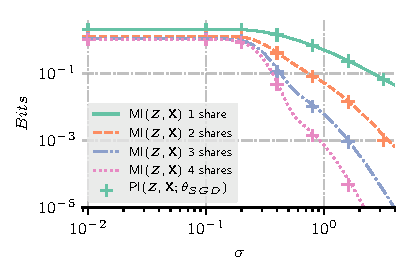
\includegraphics{Figures/simus/MI_bool_exp1_05}
        \caption{Experiment 1}
        \label{fig:exp_MI_1}
    \end{subfigure}
    \begin{subfigure}{0.49\textwidth}
        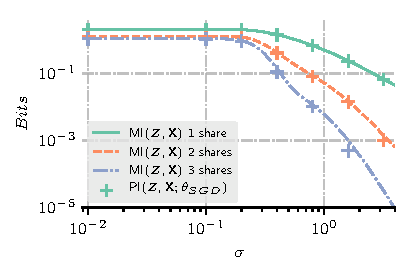
\includegraphics{Figures/simus/MI_bool_exp2_05}
        \caption{Experiment 2}
        \label{fig:exp_MI_2}
    \end{subfigure}
    \begin{subfigure}{0.49\textwidth}
        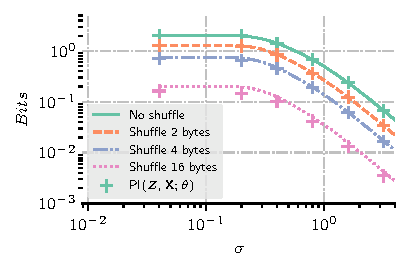
\includegraphics{Figures/simus/shuffle_simus}
        \caption{Experiment 3}
        \label{fig:exp_MI_3}
    \end{subfigure}
	\caption{Information perceived by the \gls{mlp}.}
	\label{fig:exp_MI}
\end{figure}


In this section we analyze the results obtained by running Experiments \(1\) (\autoref{fig:exp_MI_1}), \(2\) (\autoref{fig:exp_MI_2}) and \(3\) (\autoref{fig:exp_MI_3}).
On each figure, the lines correspond to the estimated \gls{mi} and the crosses correspond to the information perceived by the trained \gls{mlp}, as computed from the \gls{nll} loss with \autoref{eq:PI_eq_gen_loss}.
Based on these results, several observations can be done.

First, on each result the crosses are always below the lines, which is in line with the results given in the literature: the estimated \gls{pi} is a lower bound of the \gls{mi}. 
But more interestingly, the crosses are always close to the line no matter the \gls{mi} magnitude.
In the case of Experiment 1, we argued that the error was composed of the approximation and optimization errors, so their sum is negligible.
Since we recalled in \autoref{sec:div_term} that those terms are both negative, we conclude that even for a simple \gls{mlp} with one layer and \(1,000\) neurons, both errors can be ignored. 
This is of particular interest concerning the approximation error, as it always decreases with the number of layers and the number of neurons inside each layer of the \gls{mlp}. 
Therefore, in the case of a Hamming weight leakage model with additive Gaussian noise, any \textit{more sophisticated} \gls{mlp} (\ie{} with more layers or more neurons by layer) will also have a negligible approximation error.

Secondly, the \gls{pi} plotted in \autoref{fig:exp_MI_2} shows that the presence of uninformative components in Experiment 2 does not annihilate the capacity of the \gls{mlp} to optimally extract information about the target variable, provided that these components are not shuffled with informative ones.
This shows that the optimization error, which was thought to be increased compared to Experiment 1, remains stable.

Finally, the preceding observations hold regardless the considered counter-measure, namely secret-sharing (\autoref{fig:exp_MI_1} and \autoref{fig:exp_MI_2}) or shuffling (\autoref{fig:exp_MI_3}).
This can be interpreted as the fact that the \gls{mlp} trained through the \gls{nll} loss minimization is able to give a model optimally extracting the remaining informative leakage, while being ``agnostic'' concerning the presence or not of such counter-measures.
Nevertheless, since both counter-measures have been shown to decrease the \gls{mi} -- exponentially with the level of noise for secret-sharing as explained in \autoref{sec:masking} or linearly for shuffling as explained in \autoref{sec:hiding} -- they remain sound against Deep Learning.

At this stage, we have argued thanks to our simulations that the approximation error is negligible, no matter the considered counter-measure, nor the architecture of a \gls{mlp}, while the optimization error is likely to remain negligible as well.
Therefore, our \gls{mi} estimation obtained by \gls{pi} maximization seems accurate. 
This provides an empirical validation of \autoref{prop:cor_sup_PI}.
As another consequence, we are fairly confident that in the case of such simple leakage models, which often happen on real use cases, replacing an optimal architecture by another should not degrade too much the \gls{mi} estimation.%
\footnote{However, one cannot get such a conclusion if one considers another leakage model.}
These observations must be challenged by tests on experimental traces, where one cannot have an exhaustive dataset. 
This will naturally lead to discussions regarding the estimation error which has not been investigated here.

\section{Application on Experimental Data}
    \label{sec:experiments}
    So far, we have seen that \glspl{dnn} could reach the informational security bounds of a leakage in simulated experiments, thereby giving useful estimations for the developer.
    This success did not rely on any prior knowledge on the leakage, but was achieved thanks to a simple \gls{mlp} with one hidden layer. 
    To confirm these observations, we propose to complete the investigations by considering experimental leakage traces from the \textsf{Chip Whisperer} dataset presented in \autoref{sec:dataset_cw}.
    \autoref{sec:exp_method} presents the methodology of our experiments, and \autoref{sec:results_exp} discusses their results.

\subsection{Methodology}
    \label{sec:exp_method}
    %%%%%%%%%%%%%%%%%%%%%%%%%%%%%%%%%%%%%%%%%%%%%%%%%%%%%%%%%%%%%%%%%%%%%%%%%%%%%%%%
%                           METHODOLOGIE CHES                                  %
%%%%%%%%%%%%%%%%%%%%%%%%%%%%%%%%%%%%%%%%%%%%%%%%%%%%%%%%%%%%%%%%%%%%%%%%%%%%%%%%
\paragraph{The hypothesis class \(\hypoclass\).}
The hypothesis class \(\hypoclass\) used for the next two experiments, namely Experiments 4 and 5, is defined as the set of \gls{mlp} with \(\numLayers=1\) hidden layer and \(\linSize = 500\) hidden neurons.
That is,
\begin{equation}
    \MLmodel = s \circ \linLayer_2 \circ \BNLayer \circ
    \dropLayer_q \circ \actLayer \circ \linLayer_1 \circ \BNLayer \enspace ,
  \end{equation}
where \(\dropLayer_q\) denotes a dropout layer of parameter \(q\), compared to the architecture presented in \autoref{sec:pres_architectures}.
The dropout parameter has been set to \(q=0.1\) \ie{} each neuron of the hidden layer is randomly set to \(0\) with probability \(q\) each time an output \(\MLmodel(\xxx)\) is computed during the optimization.

\paragraph{Common settings.}
The trainings have been done with the \gls{adam} algorithm through a number of epochs denoted by \(T\), \ie{}, each trace has been processed \(T\) times by the algorithm. 
Over the \(500,000\) profiling traces, a portion \(\alpha\) is used for the training, and the remaining is used as a hold-out set for computing an unbiased estimate of the perceived information. 
In other words, the profiling set is made of \(\numTracesProf = \alpha \times 500, 000\) traces while the hold-out set is made of \(\numTracesVal = (1 - \alpha) \times 500,000\) traces.
We fix the limit \(\alpha \leq 4/5\) so that the quality of the estimation over the hold-out set remains satisfying: the error margin will be at most \(10^{-2}\) with a confidence at least \(90 \%\) in the worst case, according to Chebyshev's inequality -- see \autoref{sec:probas}.


\paragraph{Experiment 4 on Boolean secret-sharing.}
When considering secret-sharing, the generated target values are \(\Z = \bigoplus_{j \in \llbracket 0, \order \rrbracket} \verb+plain+[j]\) for \(\order \in \{0, 1, 2\}\), where \(\oplus\) denotes the \verb+xor+ operation between two bytes. 
This way, it can simulate leakages of order \(\order\).

Provided with these target values, we selected \glspl{poi} based on the magnitude of the \gls{snr}: between 4 and 6 \glspl{poi} are selected in decreasing order of magnitude of \gls{snr} from each of the three first bytes of the plaintext array -- see \autoref{fig:snr_cw}.
The time coordinates \(13\) to \(16\), \(25\) to \(30\) and \(37\) to \(41\) correspond respectively to the \glspl{poi} of the latter bytes manipulation. 
This gives an input dimension of \(\traceLength = 15\).
This way, we hoped to reduce the quantity of irrelevant components, which would have made the optimization with \gls{adam} harder, and therefore hoped to get a good estimate corresponding the most to the approximation error~\eqref{eq:err_approx_ches}.
Details of the trained \gls{mlp} can be found hereafter.
We set \(T = 200\) and let \(\alpha\) vary so that \(\card{\trainSet} \in \llbracket 1,000; 400,000\rrbracket\). 
This way, we will be able to plot the so-called \emph{learning curve}, namely plotting the values of \(\PI{\Z}{\XXX}{\MLmodelSGD{\trainSet}}\) and \(\estPI{\Z}{\XXX}{\MLmodelSGD{\trainSet}}{\card{\trainSet}}\) depending on \(\card{\trainSet}\).
This is a classical representation in machine learning.
On a learning curve, it is expected that the empirical \gls{pi} decreases with \(\card{\trainSet}\) while the true \gls{pi} increases, and both converge towards the supremum of the \gls{pi}~\cite{vapnik_nature_1995}.
This representation enables to discuss the estimation error~\eqref{eq:err_est_ches} according to the size of the profiling set.


\paragraph{Experiment 5 on shuffling.}
When considering shuffling, the generated target values are \(\Z = \verb+plain+[j]\) where \(j\) is randomly drawn from a subset of \(\llbracket 0, 15 \rrbracket\) of size \(\shufflingOrder\), \(\shufflingOrder\) denoting the number of shuffled bytes.

Contrary to the experiments on secret-sharing, we did not selected \glspl{poi} but only restricted the target window to the \(\traceLength = 250\) first time samples of the traces, which was sufficient to cover the leakages of every shuffled plaintext byte (see \autoref{fig:snr_cw}).
Afterwards, a \gls{cnn} with a \gls{vgg}-like architecture has been used for those trainings.

We set \(\alpha = 4/5\), \(T = 100\), and \(\shufflingOrder \in \{1, 2, 4, 16\}\).
The aim of this experiment is to empirically verify the trend observed on the Experiment 3 (\autoref{fig:exp_MI_3}), namely a linear decrease of \gls{pi} with the number of shuffled bytes.

\subsection{Results and Discussions}
    \label{sec:results_exp}
    %%%%%%%%%%%%%%%%%%%%%%%%%%%%%%%%%%%%%%%%%%%%%%%%%%%%%%%%%%%%%%%%%%%%%%%%%%%%%%%%
%                           RESULTS DATASET CW CHES                          %
%%%%%%%%%%%%%%%%%%%%%%%%%%%%%%%%%%%%%%%%%%%%%%%%%%%%%%%%%%%%%%%%%%%%%%%%%%%%%%%%
\begin{figure}
    \centering
    \begin{subfigure}{0.49\textwidth}
        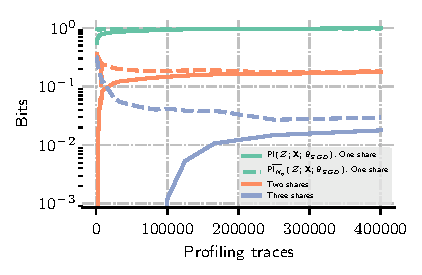
\includegraphics{Figures/experiments/learning_curves_05}
        \caption{Learning curve of Experiment 4 on Boolean secret-sharing.}
        \label{fig:exp_PI_4}
    \end{subfigure}
    \begin{subfigure}{0.49\textwidth}
        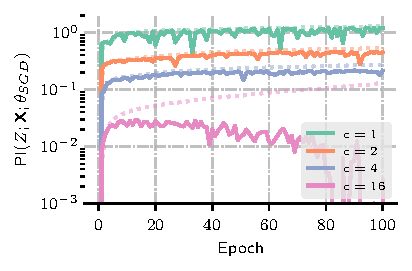
\includegraphics{Figures/experiments/PI_shuffle_4_bits}
        \caption{Results of Experiment 5 on shuffling.}
        \label{fig:exp_PI_5}
    \end{subfigure}
    \caption{Results on experimental data.}
    \label{fig:exp_PI}
\end{figure}
\autoref{fig:exp_PI_4} presents the learning curves of Experiment 4, when targeting respectively \(1, 2\) or \(3\) shares among the considered ones.
The dotted curves are the estimated \gls{pi} over the \(\numTracesProf = \card{\trainSet}\) profiling traces whereas the plain curves denote the \gls{pi} estimated with the \(\numTracesVal\) validation traces.
  
It may first be observed that the amount of information leaking on the sensitive un-split variable seems to decrease at an exponential rate in the number of shares, as expected from both theory -- see \autoref{sec:masking} -- and our simulations -- see \autoref{sec:simus}.
More interestingly, the gap between dotted curves and their corresponding plain ones exactly corresponds to the estimation error term~\eqref{eq:err_est_ches}.
It appears then that the latter one becomes negligible relatively to the \gls{pi} when the profiling set size exceeds respectively a few thousands when targeting one share, or one hundred thousand when targeting two shares.
When targeting three shares, the estimation error is not completely negligible, even with \(400,000\) profiling traces.
It is furthermore particularly noticeable that when profiling the three shares scheme with less than \(100,000\) traces, the learning phase completely failed since the \gls{pi} was null. 
This indicates that, in addition to the effect on \gls{mi} predicted by theoretical works, the secret-sharing counter-measure also has an effect on the \gls{pi} through an increasing estimation error, making the \gls{mi} estimation poorer.
  
  
\autoref{fig:exp_PI_5} presents the results of Experiment 5 on shuffling. 
It is recalled that contrary to Experiment 4 where \glspl{poi} where extracted, here \(250\)-dimensional traces have been processed through a \gls{dnn}. 
The gap in \autoref{fig:exp_MI_3} between each curve remains observable on \autoref{fig:exp_PI_5} when considering experimental traces.
However, the \gls{pi} obtained when the attack target is shuffled among \(16\) random values seems decreasing starting the \(20\)-th epoch, while the empirical \gls{pi} (in dotted curves) keeps increasing.
This is a sign of \emph{over-fitting}.

% Over-fitting
Indeed, if the estimation error is high, the optimization algorithm is expected to return at each iteration a better model with respect to the training loss \(\LossFunc[\trainSet]{}\).
Since the latter one is different from the cross entropy \(\LossFunc[\XXX, \Z]{}\), an improvement with respect to the training loss may not be an improvement with respect to the cross entropy, or equivalently, with respect to the \gls{pi}.
That is why there is a moment when the loss computed over the validation traces starts increasing whereas the training loss keep decreasing.
In other words, the model starts to learn \emph{by heart} to build its prediction on some uninformative features which would not generalize well during the attack phase on unknown traces.
The higher the estimation error, the less similar the \gls{nll} loss and the cross entropy so the sooner and the more importantly over-fitting happens.
Therefore, the \gls{pi} reached in the graph is not necessarily optimal: more profiling traces might be required to decrease the estimation error and thereby mitigating the effect of over-fitting.

Altogether, our experiments show that similarly to the approximation and optimization errors discussed in \autoref{sec:simus}, the estimation error is also negligible relatively to the \gls{mi}, when considering unprotected scenarios where the profiling set size is reasonably high (\ie{} \(10,000\) traces or above). 
This therefore leads to a tight estimation of the \gls{mi} through the maximization of the \gls{pi} (\ie{} the minimization of the \gls{nll} loss).
When considering protected devices, the investigated counter-measures impact the estimation error, and thereby the tightness of the lower bound computed through \gls{pi} maximization.
Nevertheless this can be controlled by increasing the size of the profiling set.
More precisely, the \textit{harder} the counter-measure (\ie{} the higher the sharing order, or the more shuffled bytes), the higher the profiling set size.
  
  
Another way to decrease the estimation error would be to decrease the \textit{capacity} of the hypotheses class, \ie{} its \gls{vc}-dimension, by decreasing the number of layers or the number of neurons on each layer. 
Since we have argued in \autoref{sec:analysis_simus} that the approximation error was negligible even for a simple architecture, we are quite confident that this would not strongly affect the quality of the \gls{mi} estimation.

\subsection{Application on Public Datasets}
    \label{sec:experiments_datasets}
    %%%%%%%%%%%%%%%%%%%%%%%%%%%%%%%%%%%%%%%%%%%%%%%%%%%%%%%%%%%%%%%%%%%%%%%%%%%%%%%%
%                       EXPERIMENT DATASETS CHES                               %
%%%%%%%%%%%%%%%%%%%%%%%%%%%%%%%%%%%%%%%%%%%%%%%%%%%%%%%%%%%%%%%%%%%%%%%%%%%%%%%%
So far, we have considered our experimental investigations through the view of the Leakage Assessment Problem (\ie{} \autoref{leak_assess}).
However, we remind that the final task an evaluator is given to achieve is the profiled \gls{sca} optimization (\ie{} \autoref{final_task_prof}), namely to find \(\numTracesAttackOpt\).

It is recalled that \autoref{cor:main_result} argued that by solving the Leakage Assessment Problem, one could get an accurate estimation \(\numTracesAttackEst{\MLmodelMLE{\trainSet}}\) of the quantity \(\frac{f(\beta)}{\MI{\Z}{\XXX}}\), known to be a lower-bound of the optimal solution of the profiled \gls{sca} optimization problem, namely \(\numTracesAttackOpt\).

One could wonder whether this inequality still holds for any model, maybe sub-optimal, \ie{} when estimating the minimal number of queries \(\numTracesAttack(\MLmodel)\) to the target device for such a model with the quantity \(\numTracesAttackEst{\MLmodel}\).
A formal proof would be a promising further work, though beyond the scope of this thesis.%
\footnote{
    We discuss in \autoref{sec:ccl_ches} the recent improvements proposed following this work.
}
Nevertheless we propose here to empirically verify this hypothesis by training a \gls{cnn} on all the public datasets presented in \autoref{sec:datasets} and by implementing the key enumeration in order to evaluate \(\numTracesAttack(\MLmodel)\).%
\footnote{
    See the method described in \autoref{sec:estimate_practice} for the practical estimation of \(\numTracesAttack(\MLmodel)\).
}
This way, our claim can be tested under several cases covering all the counter-measures considered in this thesis.

\paragraph{Settings.}
For each training, a \gls{vgg}-like \gls{cnn} architecture has been used, as presented in \autoref{sec:pres_architectures}.
More specifically:
\begin{itemize}
    \item \textbf{\gls{ascad} and \gls{aeshd}}:
    the following parameters have been used: \(n_1 = 2\), \(n_2 = 7\), the convolutional filters are of length \(\ksize=11\) and the pooling stride is \(\pstride=2\).
    \(\numFilters = 10\) filters are in the first layer, and they are doubled at each convolutional layer.
    The last pooling layer has a stride set so that the output size along the time dimensionality is one.
    The dense layers contains \(1,000\) intermediate neurons.
    This architecture is based on our works presented at \textsc{Cosade}'19 and is more thoroughly discussed in \autoref{sec:with_mask_no_desynchro}
    \item \textbf{\gls{aesrd}}: the same \gls{vgg}-like architecture as the one presented by Kim \etal{}~\cite{kim_make_2019} has been used.
    More specifically, \(n_2\) is set to \(9\) so that there is enough pooling layers to get feature maps on the last convolutional layer whose width equals one.
    Besides, \(n_1=0\), \ie{} there is no intermediate dense layer, except softmax.
    \item \textbf{Polymorphism}: the precise architecture used for the experiments is the one used in our works presented at \textsc{Esorics}'20 and a whole dedicated discussion is proposed in \autoref{sec:cnn_archi_esorics}.
\end{itemize}

The training has been run on \(200\) epochs on the \gls{aesrd} and the Polymorphism datasets, \(50\) epochs on the \gls{aeshd} dataset, and stopped after \(30\) epochs on the \gls{ascad} dataset -- see an explanation in \autoref{sec:with_mask_no_desynchro}.
After each epoch \(t\) the optimization algorithm -- \gls{adam} here -- returns an update of the learning parameter vector denoted by \(\MLparam_t\).
We can therefore estimate the efficiency of the -- partially optimized -- model \(\MLmodel(\cdot, \MLparam_t)\), \ie{} \(\numTracesAttack\left(\MLmodel(\cdot, \MLparam_t)\right)\) thanks to a key enumeration, according to the procedure detailed in \autoref{sec:estimate_practice}.

\begin{figure}
    \centering
    \begin{subfigure}{0.49\textwidth}
        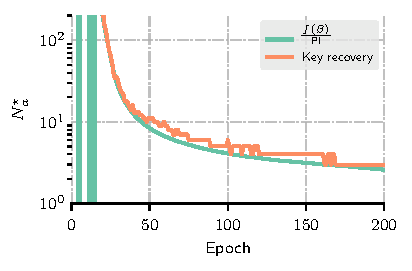
\includegraphics{Figures/experiments/RD_demo}
        \caption{\gls{aesrd} dataset.}
        \label{fig:ches_aes_rd}
    \end{subfigure}
    \begin{subfigure}{0.49\textwidth}
        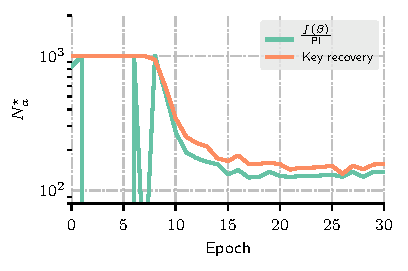
\includegraphics{Figures/experiments/ASCAD_demo}
        \caption{\gls{ascad} dataset}
        \label{fig:ches_ascad}
    \end{subfigure}
    \begin{subfigure}{0.49\textwidth}
        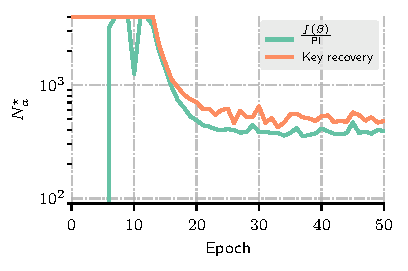
\includegraphics{Figures/experiments/AES_HD_demo}
        \caption{\gls{aeshd} dataset}
        \label{fig:ches_aes_hd}
    \end{subfigure}
    \begin{subfigure}{0.49\textwidth}
        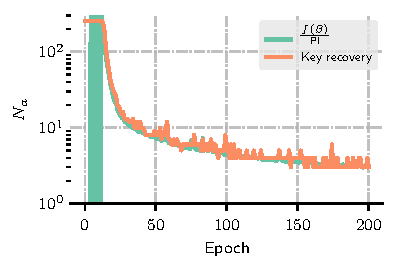
\includegraphics{Figures/experiments/mbedTLS}
        \caption{Polymorphism dataset (\mbedTLS{})}
        \label{fig:ches_mbedTLS}
    \end{subfigure}
    \begin{subfigure}{0.49\textwidth}
        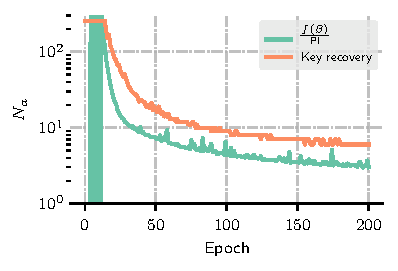
\includegraphics{Figures/experiments/aes_8bit_05}
        \caption{Polymorphism dataset (\aeshuitbit{})}
        \label{fig:ches_aes_8bit}
    \end{subfigure}
    \caption{Comparison between the estimation of \(\numTracesAttack(\MLmodel(\cdot, \MLparam_t))\) through the lower bound (orange lines) and through a key enumeration (green lines).}
    \label{fig:exp_pub_datasets}
\end{figure}

\paragraph{Results.}
The results are given in \autoref{fig:exp_pub_datasets}.
On each graph, \(\numTracesAttackEst{\MLmodel(\cdot, \MLparam_t)}\) is denoted in green, whereas the enumeration key estimation \(\numTracesAttack(\MLmodel(\cdot, \MLparam_t))\) is denoted by the orange curve.
Each curve has been clipped in order to be in \([0, 10^3]\), except for the \gls{aeshd} dataset where the high threshold is \(4.10^3\) since the literature presumed a higher \(\numTracesAttackOpt\)~\cite{kim_make_2019,zaid_methodology_2019}.


On \autoref{fig:ches_aes_rd}, we can remark that the first epochs of the profiling of the \gls{aesrd} dataset show a chaotic behavior.
This is explained by the fact that the \gls{nll} loss is initially close to \(n=8\) bits, or in other words, the \gls{pi} is close to zero, leading to unstable estimations of \(\numTracesAttackEst{\MLmodel(\cdot, \MLparam_t)}\). 
Once the model has started extracting some information, \ie{} after approximately epochs, the \gls{pi} starts to be significantly higher than \(0\) and the unstability vanishes. 
We can then observe that \(\numTracesAttackEst{\MLmodel(\cdot, \MLparam_t)}\) is always lower than the key enumeration estimation \(\numTracesAttack(\MLmodel(\cdot, \MLparam_t))\) as expected, while remaining tight through the epochs: the average relative error, computed starting the \(t=20\)-th epoch is of \(16\%\).
The final model is able to recover the secret key in \(3\) traces, and has a \gls{pi} of \(2.95\) bits/trace.%
\footnote{
    Those results coincide with the ones reported by Kim \etal{}~\cite{kim_make_2019}.
}

Likewise, for the \gls{ascad} dataset, the results are presented in \autoref{fig:ches_ascad}.
We can observe the same unstability at the beginning of the training, though the quantity \(\numTracesAttackEst{\MLmodel(\cdot, \MLparam_t)}\) remains lower than the estimation through the enumeration key afterwards, while staying quite tight.
The average relative error is also here of \(16\%\), and the final \gls{pi} is \(0.065\) bit/trace.

In addition, for the \gls{aeshd}, the results are presented in \autoref{fig:ches_aes_hd}.
Similarly to the two preceding experiments, a tight estimation is obtained, since the relative error is \(18\%\), while the final \gls{pi} is \(0.020\) bit/trace.

Finally, the outcomes on the two Polymorphism datasets are presented.
\autoref{fig:ches_mbedTLS} deals with the \mbedTLS{} implementation and depicts two superposed curves, hence a tight estimation of \(\numTracesAttack(\MLmodel(\cdot, \MLparam_t))\).
Similarly, \autoref{fig:ches_aes_8bit} deals with the \aeshuitbit{} implementation.
Although the estimation seems looser, the relative error remains of \(15\%\).

As a consequence, all those experiments tend to confirm that the quantities \(\numTracesAttackEst{\MLmodel(\cdot, \MLparam_t)}\) and \(\numTracesAttack(\MLmodel(\cdot, \MLparam_t))\) are effectively related, at least for a threshold \(\beta = 90\%\).
This is of great interest in the evaluation of the security of a device, since this not only empirically shows the relevance of minimizing the \gls{nll} loss, but this also provides a relevant tool to predict the required number of queries to succeed the key recovery, or at least to give a lower-bound to such a number, which is still useful since we look for a worst case scenario in a \gls{sca} evaluation.

\section{Conclusion}
    \label{sec:ccl_ches}
    %%%%%%%%%%%%%%%%%%%%%%%%%%%%%%%%%%%%%%%%%%%%%%%%%%%%%%%%%%%%%%%%%%%%%%%%%%%%%%%%
%                           CONCLUSION CHAPTER 5                               %
%%%%%%%%%%%%%%%%%%%%%%%%%%%%%%%%%%%%%%%%%%%%%%%%%%%%%%%%%%%%%%%%%%%%%%%%%%%%%%%%
In this chapter, we have given some theoretical and experimental reasons why the deep learning paradigm is suitable for evaluating implementations against \gls{sca} 
from a worst-case scenario point of view, regardless the nature of the counter-measures.

Contrary to what was commonly believed until the works of Picek \etal{}~\cite{picek_curse_2019}, the supervised classification approach is not theoretically grounded generally speaking as discussed in \autoref{chap:machine_learning}.
Yet, deep learning based attacks still worked.
The reason is that in the specific case where the \gls{nll} is used as a surrogate loss function, it turns out that the latter one is actually consistent with maximizing the \gls{pi}, solving the so-called Leakage Assessment Problem.
Since the latter problem was argued to be sound with the profiled \gls{sca} optimization problem, we conclude that the choice of the \gls{nll} as a surrogate loss function is sound from an evaluation point of view, in the sense that it enables to accurately estimate a lower bound of the minimal number of queries required by an attacker provided with an optimal leakage model in order to successfully recover the secret key.

Simulations and experiments verified that the \gls{pi} maximization via \gls{nll} minimization was an efficient method in order to estimate the \gls{mi} in several configurations, \ie{} on different architectures and with different types of counter-measures, including higher order secret-sharing, shuffling or de-synchronization through random delays.

This leads to the takeaway messages of this chapter: the minimization of the \gls{nll} loss via a neural network model enables to give relevant estimations of the mutual information between a sensitive variable and the corresponding side-channel traces, thereby quantitatively measuring the impact of counter-measures (and their implementations) so that an evaluator can precisely assess whether the latter one stays sound or not.

% About the HI
A possible track of work following the study presented in this chapter could investigate how \gls{dl} could also be used to estimate the \gls{hi}, another information theoretic notion extending the \gls{mi} and the \gls{pi}.
Bronchain \etal{} considered this metric as well in their paper at \textsc{Crypto}'19 and showed that it is an upper-bound of the \gls{mi} whereas the \gls{pi} is a lower bound.
It would be interesting to know whether there is a way to \emph{minimize} the \gls{hi} of an approximate leakage model, in order to get an insightful confidence interval of the \gls{mi}, along with the \gls{pi}.
Unfortunately, the computation of \gls{hi} would rely on generative models, beyond the scope of this thesis.
Yet, investigating whether there are sound generative \gls{dl} models in an \gls{sca} context could be promising.


\paragraph{Epilogue.}
Since the release of our paper at \textsc{Ches} 2020, two recent works have addressed the problem of the choice of the loss function, following our line of works.

Zhang \etal{} have proposed a slight variant of the \gls{nll}~\cite{zhang_novel_2020}.
According to the authors, the latter loss function would have a major drawback when dealing with datasets for which the observed values of the sensitive variable are not uniformly distributed, \eg{}, if one targets \(\Z' = \hWeight(\Z)\) instead of \(\Z\).
If the precise distribution \(\prob{\Z'}\) is unknown, then so is \(\entrop{\Z'}\), which means that one cannot compute the \gls{pi}.
Nevertheless, one can still maximize it, since the unknown term does not depend on the considered model \(\MLmodel\) with respect to which the optimization is done.
To circumvent this problem, the authors propose the \gls{cer}, which is the ratio between the \gls{nll} computed for the right key hypothesis, and the average of the \glspl{nll} computed when assuming any other wrong key hypotheses.
They show that an attack is effective \gls{iff} this metric is below \(1\).
Moreover, they claim that the lower the metric, the more efficient the attack, which is empirically verified on several public datasets.
Yet, a formal proof of this trend still remains to be established.

% Ranking loss
Zaid \etal{} have recently embraced another approach when tackling the issue of the loss function, leading to proposing the so-called \emph{ranking} loss~\cite{zaid_ranking_2020}.
Contrary to the \gls{nll} coming from the supervised classification task, the authors here take inspiration from another learning task, namely \emph{learning to rank}.
By translating this task into the profiled \gls{sca} optimization framework, they show the soundness of their approach to maximize the \gls{sr}.

Beyond being useful for estimating the \gls{sca} efficiency metric, the computation of the \gls{mi} could be a goal as itself for the evaluator~\cite{bronchain_leakage_2019}.
Hence, Cristiani \etal{} recently extended a technique called \emph{Neural Estimation of the Mutual Information}, originally introduced by Belghazi \etal{}~\cite{belghazi_mine_2018}, in the aim to derive the best way to to estimate the \gls{mi} between \gls{sca} traces and a sensitive intermediate computation~\cite{cristiani_leakage_2020}.